% !TEX TS-program = XeLaTeX
% !TEX encoding = UTF-8 Unicode

\chapter{图表、公式及参考文献的使用说明}
\label{chap02}

这里给出一些例子用来说明图表和公式的使用。

    \section{图}
    \label{chap02:figure}
    下图~\ref{fig:chap02:manner}~是Word的模版中使用的图片,这里用来做个例子。

    \begin{figure}[!htbp]
        \centering
        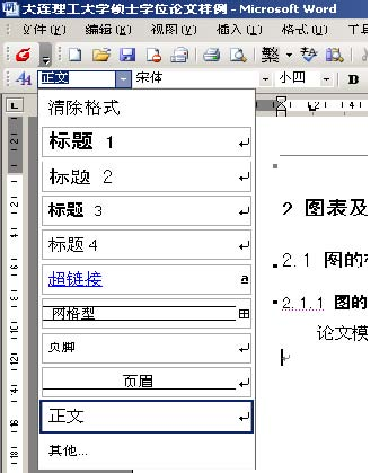
\includegraphics[scale=1]{manner.pdf}
        \bicaption[fig:chap02:manner]{样式}{样式}{Fig.}{Manner}
    \end{figure}

    它的源代码如下:
\begin{Verbatim}[fontsize=\footnotesize, frame=single, baselinestretch=1]
    \begin{figure}[!htbp]
    \centering
    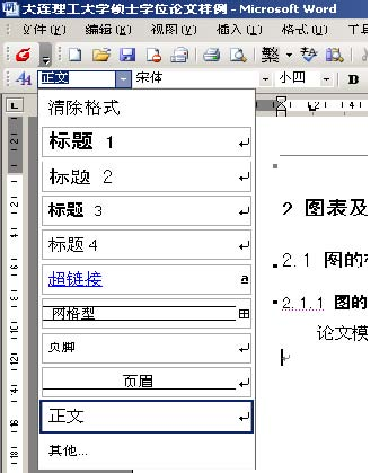
\includegraphics[scale=1]{manner.pdf}
    \bicaption[fig:chap02:manner]{样式}{样式}{Fig.}{Manner}
    \end{figure}
\end{Verbatim}

    其中标题使用的是ccaption宏包的~\texttt{\footnotesize bicaption}~命令,可以显示中英文双标题。
    它的官方使用说明为:
\begin{Verbatim}[fontsize=\footnotesize, frame=single, baselinestretch=1]
    \bicaption[<label>]{<short-1>}{<long-1>}{<NAME>}{<long-2>}
\end{Verbatim}
    可选参数~\texttt{\footnotesize <label>}~用来作为引用链接。
    \texttt{\footnotesize <short-1>}~和~\texttt{\footnotesize <long-1>}~分别是主语言(这里指汉语)的短标题和长标题。
    \texttt{\footnotesize <NAME>}~是次语言(这里指英语)的标题名称,按要求固定为Fig.。
    最后一个参数~\texttt{\footnotesize <long-2>}~表示次语言的标题。

    注意到标题的位置必须位于图片的下方,所以使用时标题的代码也必须在插图的代码之后。

    其他插图问题请参考《{\LaTeX 2$\varepsilon$}~插图指南》\ucite{WANG00}。

    测试一下文献引用\ucite{WRH-SPLBOK94}。

    \section{表}
    \label{chap02:table}

    还是先给出官方的例子。

    物流的概念和范围如表~\ref{tab:chap02:logistics}~表述。

    \begin{table}[h]
        \bicaption[tab:chap02:logistics]{物流的概念和范围}{物流的概念和范围}{Tab.}{Conception and scope of Logistics}
        \centering
        \vspace{0.2cm}
        \dawu
        \begin{tabular}{cc}
        \hline
        {\hei 本质} & {\hei 过程}\\
        \hline
        途径或方法 & 规划、实施、控制\\
        目标 & {效率、成本效益}\\
        活动或作业 & 流动与储存\\
        处理对象 & 原材料、在制品、产成品、相关信息\\
        范围 & 从原点(供应商)到终点(最终顾客)\\
        目的或目标 & 适应顾客的需求(产品、功能、数量、质量、时间、价格)\\
        \hline
        \end{tabular}
    \end{table}

    它的源代码为:
\begin{Verbatim}[fontsize=\small, frame=single, baselinestretch=1]
    \begin{table}[h]
        \bicaption[tab:logistics]{物流的概念和范围}{物流的概念和范围}
        {Tab.}{Conception and scope of Logistics}
        \centering
        \vspace{0.2cm}
        \dawu
        \begin{tabular}{cc}
        \hline
        {\hei 本质} & {\hei 过程}\\
        \hline
        途径或方法 & 规划、实施、控制\\
        目标 & {效率、成本效益}\\
        活动或作业 & 流动与储存\\
        处理对象 & 原材料、在制品、产成品、相关信息\\
        范围 & 从原点(供应商)到终点(最终顾客)\\
        目的或目标 & 适应顾客的需求(产品、功能、数量、质量、时间、价格)\\
        \hline
        \end{tabular}
    \end{table}
\end{Verbatim}
    其中的~\Verb+\bicaption+~命令和插图中的一样,只是位置必须位于插入的表格之前。
    \Verb+\vspace{0.2cm}+~和~\Verb+\dawu+~是用来控制行间距的,请在插入表格时务必添加。


    \section{公式}
    仍旧以官方模版中的例子来演示。

    由于一般的文献资料中所给出的载荷和抗力的统计参数主要为变异系数,
    为便于讨论,定义公式形式如下:
    \begin{equation}
    \label{equ:chap02:ex1}
        LRI = \dfrac{1}{\sqrt{1+{\left(\dfrac{\mu_R}{\mu_S}\right)}^2{\left(\dfrac{\delta_R}{\delta_S}\right)}^2}}
    \end{equation}
    其中,$\mu_R,\mu_S$分别为抗力和载荷效应的均值,……。

    可以添加以上公式的引用,公式~(\ref{equ:chap02:ex1})。

    公式的使用没有什么特别的地方,注意引用公式必须使用~\Verb+\ref{}+~命令就好了。
    
    $\mathbf{A},\mathcal{A},\mathfrak{A},\mathbb{A}$

    \section{参考文献}

    本模版所使用的参考文献样式是由上海财经大学的吴凯所提供的GBT7714-2005NLang的UTF-8版本。此样式参考国家标准GB/T 7714-2005,和研究生院的Word模版的要求相一致,详细的使用说明请参考文献\cite{GBT7714-2005}。 